% figure: 自控-四种标准型模拟结构图.png
% 用途：自控（现代）01-1 §1.2.1 —— 四种常用标准型（能控/能观/对角/约当）的模拟结构图对照
% 构建：..\build.ps1 -File .\ss-four-forms.tex
% 依据：01-1 的矩阵与画法要点
%   能控标准型  A_c 末行 [-a0 -a1 -a2]，B_c=[0;0;1]，C_c=[β0 β1 β2]
%   能观标准型  A_o=A_c^T，B_o=C_c^T，C_o=B_c^T=[0 0 1]
%   对角型      每个极点一条一阶支路 1/(s-λi)，输出各支路 ×ci 汇合
%   约当型      重极点 λ1 的 m 级串联、共用 λ1；单极点各一条并联支路
% 全图取三阶（约当型取 λ1 二重 + λ3 单极点）。
\documentclass[border=10pt]{standalone}
\usepackage{fontspec}
\setmainfont{Cambria}
\usepackage{unicode-math}
\setmathfont{Cambria Math}
\usepackage{tikz}
\usetikzlibrary{positioning, arrows.meta, calc}
\usepackage{ctex}

\definecolor{figink}{HTML}{1E2228}
\definecolor{figacc}{HTML}{B23020}
\definecolor{figsub}{HTML}{606874}
\definecolor{figfill}{HTML}{E8EFF8}

\begin{document}
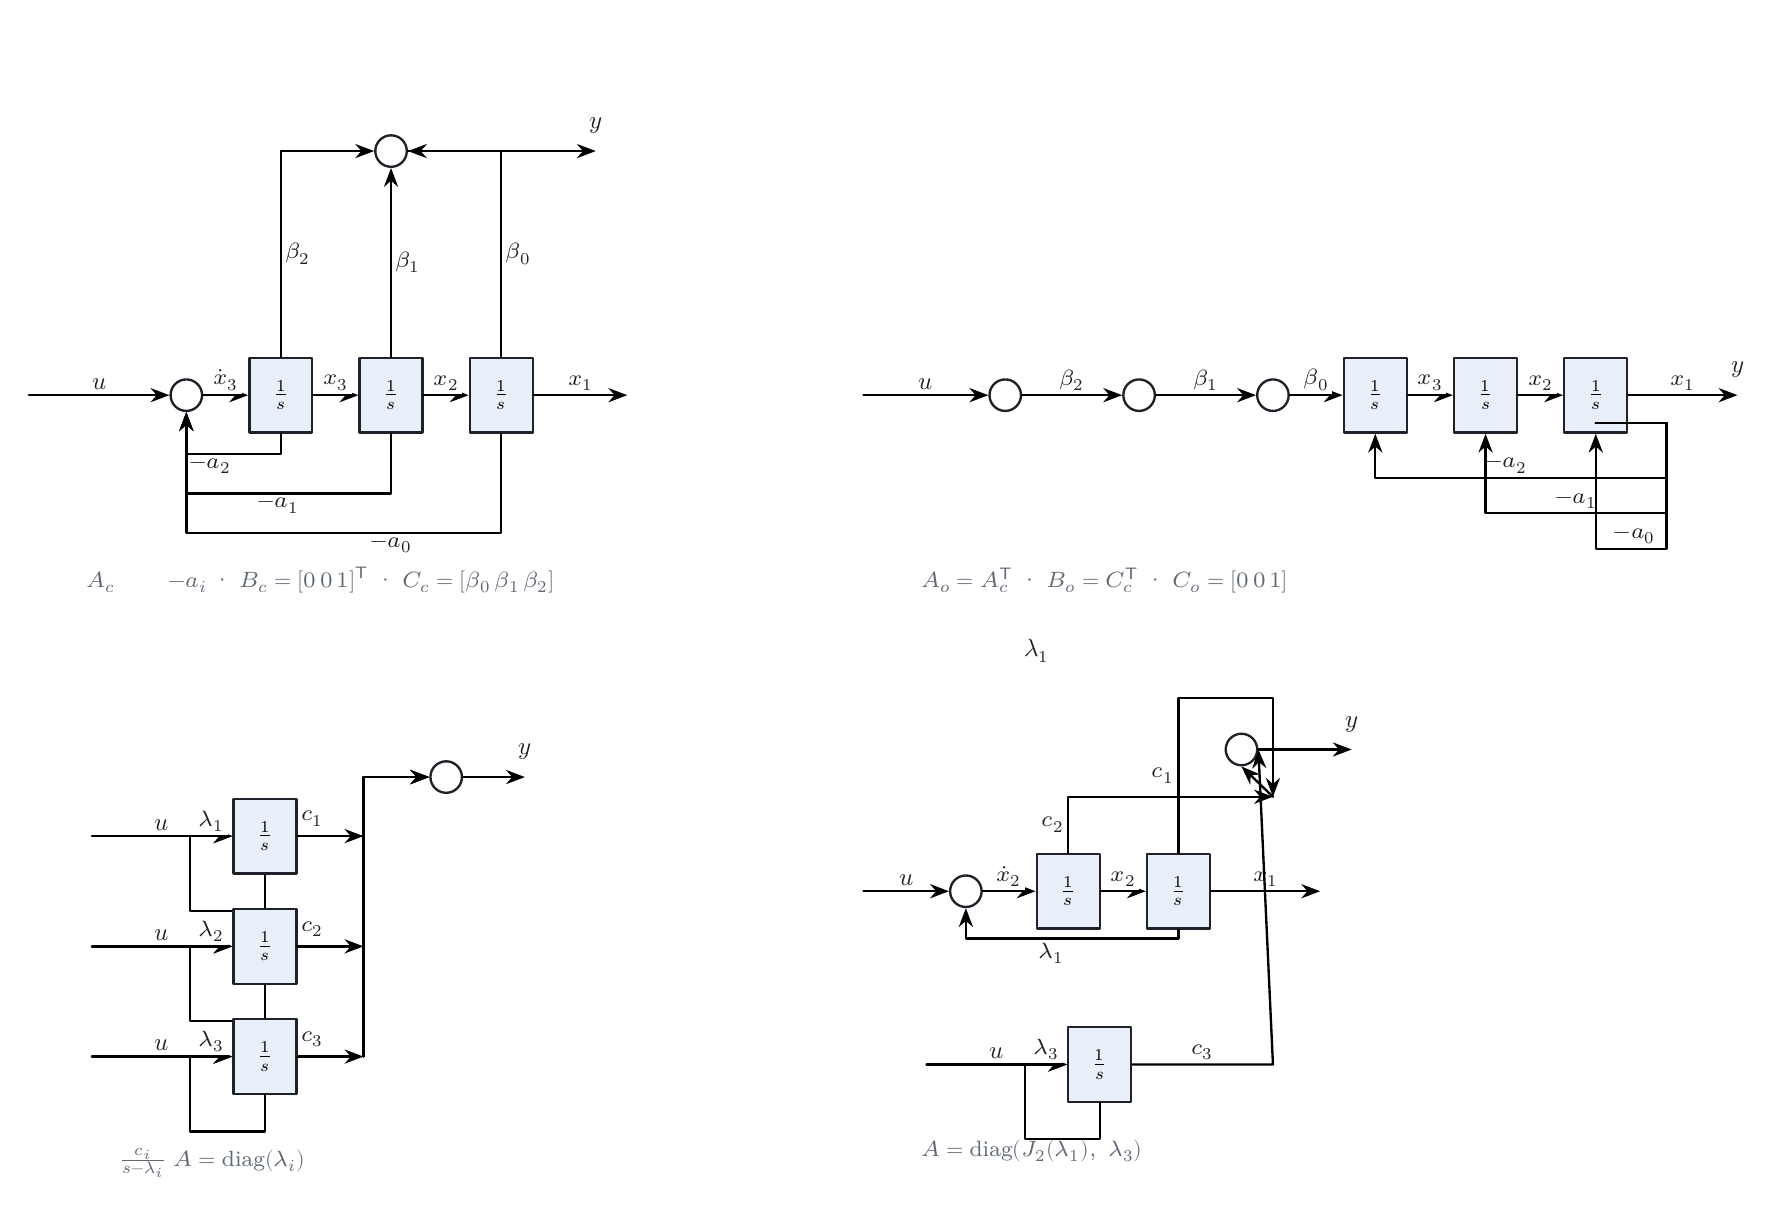
\begin{tikzpicture}[
  x=1cm, y=1cm,
  line width=0.85pt, line cap=round, line join=round,
  >=Stealth,
  sum/.style  = {draw=figink, line width=0.85pt, circle, inner sep=0pt,
                 minimum size=0.4cm, anchor=center},
  intg/.style = {draw=figink, line width=0.85pt, fill=figfill,
                 minimum width=0.8cm, minimum height=0.95cm, inner sep=1pt,
                 anchor=center, font=\small},
  sig/.style  = {font=\small, color=figink, fill=white, inner sep=1.5pt},
  g/.style    = {font=\footnotesize, color=figink, fill=white, inner sep=1.2pt},
  ttl/.style  = {font=\small\bfseries, color=figink, anchor=west},
  eq/.style   = {font=\footnotesize, color=figsub, anchor=west}
]

% ============================================================
% 左上：能控标准型
% ============================================================
\begin{scope}[shift={(0,0)}]
  \node[ttl] at (0,2.55) {① 能控标准型（串联链，输入在链首）};

  \node[sum]  (s0) at (1.4,-2.0) {};
  \node[intg] (i3) at (2.6,-2.0) {$\frac{1}{s}$};
  \node[intg] (i2) at (4.0,-2.0) {$\frac{1}{s}$};
  \node[intg] (i1) at (5.4,-2.0) {$\frac{1}{s}$};
  \node[sum]  (sy) at (4.0,1.1)  {};

  \draw[->] (-0.6,-2.0) -- node[sig, above] {$u$} (s0.west);
  \draw[->] (s0.east)   -- node[g, above] {$\dot x_3$} (i3.west);
  \draw[->] (i3.east)   -- node[g, above] {$x_3$} (i2.west);
  \draw[->] (i2.east)   -- node[g, above] {$x_2$} (i1.west);
  \draw[->] (i1.east)   -- node[g, above] {$x_1$} (7.0,-2.0);

  % 反馈：各级状态经 -a_i 汇入总线 -> 链首加法器
  \draw[->] (i3.south) -- (2.6,-2.75) -- node[g, pos=0.75, below] {$-a_2$} (1.4,-2.75) -- (s0.south);
  \draw[->] (i2.south) -- (4.0,-3.25) -- node[g, pos=0.55, below] {$-a_1$} (1.4,-3.25) -- (s0.south);
  \draw[->] (i1.south) -- (5.4,-3.75) -- node[g, pos=0.35, below] {$-a_0$} (1.4,-3.75) -- (s0.south);

  % 前馈：各阶态经 β 汇入输出加法器
  \draw[->] (i3.north) -- node[g, right] {$\beta_2$} (2.6,1.1) -- (sy.west);
  \draw[->] (i2.north) -- node[g, right] {$\beta_1$} (sy.south);
  \draw[->] (i1.north) -- node[g, right] {$\beta_0$} (5.4,1.1) -- (sy.east);
  \draw[->] (sy.east) -- (6.6,1.1);
  \node[sig] at (6.6,1.42) {$y$};

  \node[eq] at (0,-4.35) {$A_c$ 友矩阵（末行 $-a_i$）· $B_c=[0\,0\,1]^{\mathsf T}$ · $C_c=[\beta_0\,\beta_1\,\beta_2]$};
\end{scope}

% ============================================================
% 右上：能观标准型（能控图的对偶 / 转置）
% ============================================================
\begin{scope}[shift={(10.6,0)}]
  \node[ttl] at (0,2.55) {② 能观标准型（对偶：输入分布、输出取链末）};

  \node[sum]  (t1) at (1.2,-2.0) {};
  \node[sum]  (t2) at (2.9,-2.0) {};
  \node[sum]  (t3) at (4.6,-2.0) {};
  \node[intg] (j3) at (5.9,-2.0) {$\frac{1}{s}$};
  \node[intg] (j2) at (7.3,-2.0) {$\frac{1}{s}$};
  \node[intg] (j1) at (8.7,-2.0) {$\frac{1}{s}$};

  % u 经 β 分别送入各级积分器
  \draw[->] (-0.6,-2.0) -- node[sig, above] {$u$} (t1.west);
  \draw[->] (t1.east) -- node[g, above] {$\beta_2$} (t2.west);
  \draw[->] (t2.east) -- node[g, above] {$\beta_1$} (t3.west);
  \draw[->] (t3.east) -- node[g, above] {$\beta_0$} (j3.west);
  \draw[->] (j3.east) -- node[g, above] {$x_3$} (j2.west);
  \draw[->] (j2.east) -- node[g, above] {$x_2$} (j1.west);
  \draw[->] (j1.east) -- node[g, above] {$x_1$} (10.5,-2.0);
  \node[sig] at (10.5,-1.68) {$y$};

  % 各 -a_i 均取自链末 x1，分别反馈到相应积分器输入
  \draw[->] (8.7,-2.35) -- (9.6,-2.35) -- (9.6,-3.05) -- node[g, pos=0.55, above] {$-a_2$} (5.9,-3.05) -- (j3.south);
  \draw[->] (8.7,-2.35) -- (9.6,-2.35) -- (9.6,-3.5) -- node[g, pos=0.5, above] {$-a_1$} (7.3,-3.5) -- (j2.south);
  \draw[->] (8.7,-2.35) -- (9.6,-2.35) -- (9.6,-3.95) -- node[g, pos=0.45, above] {$-a_0$} (8.7,-3.95) -- (j1.south);

  \node[eq] at (0,-4.35) {$A_o=A_c^{\mathsf T}$ · $B_o=C_c^{\mathsf T}$ · $C_o=[0\,0\,1]$（输出只取链末态）};
\end{scope}

% ============================================================
% 左下：对角型
% ============================================================
\begin{scope}[shift={(0,-7.2)}]
  \node[ttl] at (0,2.35) {③ 对角型（并联一阶支路，各极点一条）};

  \node[sum]  (cy) at (4.7,0.35) {};
  % 注意：foreach 列表项不能以 / 结尾——空项会让 TikZ 解析错位，
  % 把路径里的 `--` 当成 `/` 的商，画出一条斜线。
  \foreach \k/\yy/\lam/\cf in {1/-0.4/\lambda_1/c_1, 2/-1.8/\lambda_2/c_2, 3/-3.2/\lambda_3/c_3} {
    \node[intg] (d\k) at (2.4,\yy) {$\frac{1}{s}$};
    \draw[->] (0.2,\yy) -- node[sig, above] {$u$} (d\k.west);
    \draw[->] (d\k.south) -- (2.4,\yy-0.95) -- (1.45,\yy-0.95) -- (1.45,\yy) -- node[g, above] {$\lam$} (d\k.west);
    % 支路输出先向右引出，再折向输出加法器（不要斜穿，否则会盖住标签）
    \draw[->] (d\k.east) -- (3.65,\yy);
    \node[g] at (3.0,\yy+0.22) {$\cf$};
    \draw[->] (3.65,\yy) -- (3.65,0.35) -- (cy.west);
  }
  \draw[->] (cy.east) -- (5.7,0.35);
  \node[sig] at (5.7,0.67) {$y$};

  \node[eq] at (0,-4.55) {支路传函 $\frac{c_i}{s-\lambda_i}$；$A=\operatorname{diag}(\lambda_i)$（各模态解耦）};
\end{scope}

% ============================================================
% 右下：约当型
% ============================================================
\begin{scope}[shift={(10.6,-7.6)}]
  \node[ttl] at (0,2.35) {④ 约当型（重极点串联共用 $\lambda_1$，单极点并联）};

  \node[sum]  (jy)  at (4.2,1.1) {};
  % 重极点 λ1：二级串联、共用 λ1
  \node[sum]  (js)  at (0.7,-0.7) {};
  \node[intg] (k2)  at (2.0,-0.7) {$\frac{1}{s}$};
  \node[intg] (k1)  at (3.4,-0.7) {$\frac{1}{s}$};
  \draw[->] (-0.6,-0.7) -- node[sig, above] {$u$} (js.west);
  \draw[->] (js.east) -- node[g, above] {$\dot x_2$} (k2.west);
  \draw[->] (k2.east) -- node[g, above] {$x_2$} (k1.west);
  \draw[->] (k1.east) -- node[g, above] {$x_1$} (5.2,-0.7);
  \draw[->] (k1.south) -- (3.4,-1.3) -- node[g, pos=0.6, below] {$\lambda_1$} (0.7,-1.3) -- (js.south);
  % 输出支路：先在 y=0.5 汇成一条总线，再从加法器南口进（避免与 x2/x1 标签同排）
  \draw[->] (k2.north) -- node[g, left] {$c_2$} (2.0,0.5) -- (4.6,0.5);
  \draw[->] (k1.north) -- node[g, left] {$c_1$} (3.4,1.75) -- (4.6,1.75) -- (4.6,0.5);
  \draw[->] (4.6,0.5) -- (jy.south);

  % 单极点 λ3：并联一条支路
  \node[intg] (k3) at (2.4,-2.9) {$\frac{1}{s}$};
  \draw[->] (0.2,-2.9) -- node[sig, above] {$u$} (k3.west);
  \draw[->] (k3.south) -- (2.4,-3.85) -- (1.45,-3.85) -- (1.45,-2.9) -- node[g, above] {$\lambda_3$} (k3.west);
  \draw[->] (k3.east) -- node[g, above] {$c_3$} (4.6,-2.9) -- (jy.east);
  \draw[->] (jy.east) -- (5.6,1.1);
  \node[sig] at (5.6,1.42) {$y$};
  \node[eq, align=left] at (0,-4.0) {$A=\operatorname{diag}(J_2(\lambda_1),\ \lambda_3)$：块内串联、块间并联};
\end{scope}

\end{tikzpicture}
\end{document}
